Der Pole-Zero-Plot stellt die Pole und Nullstellen der Übertragungsfunktion in der komplexen Ebene dar. Pole werden durch ein Kreuz dargestellt, Nullstellen durch einen Kreis. Ein Doppelpol wird durch ein Doppelkreuz und eine Nullstelle durch einen Doppelkreis dargestellt. Der PZP enthält keine Informationen mehr über die statische Verstärkung. Aus dem PZP lassen sich Eigenschaften wie Stabilität und Minimalphasigkeit ablesen. So ist ein System stabil, wenn alle Pole in der linken offenen Halbebene liegen. Es ist instabil, sobald ein Pol auf der rechten Halbebene liegt. Es ist grenzstabil, wenn keine Pole in der rechten Halbebene liegen aber einige auf der imaginären Achse liegen. Ein System ist minimalphasig, wenn alle Nullstellen in der offenen linken Halbebene liegen. Es ist nicht minimalphasig, sobald eine Nullstelle auf der rechten Halbebene liegt. Und letztlich ist es schwachminimalphasig, wenn keine Nullstelle auf der rechten Halbebene liegt, aber Nullstellen auf der imaginären Achse auftauchen.\\
In Matlab lässt sich der Pol-Nullstellen-Plot mit folgendem Befehl erzeugen:\\
\hspace*{0.5cm}\texttt{pzplot(sys)}\\
Das Ergebnis dieses Befehls ist in der nachfolgenden Abbildung dargestellt:
\begin{figure}[H]
    \centering
    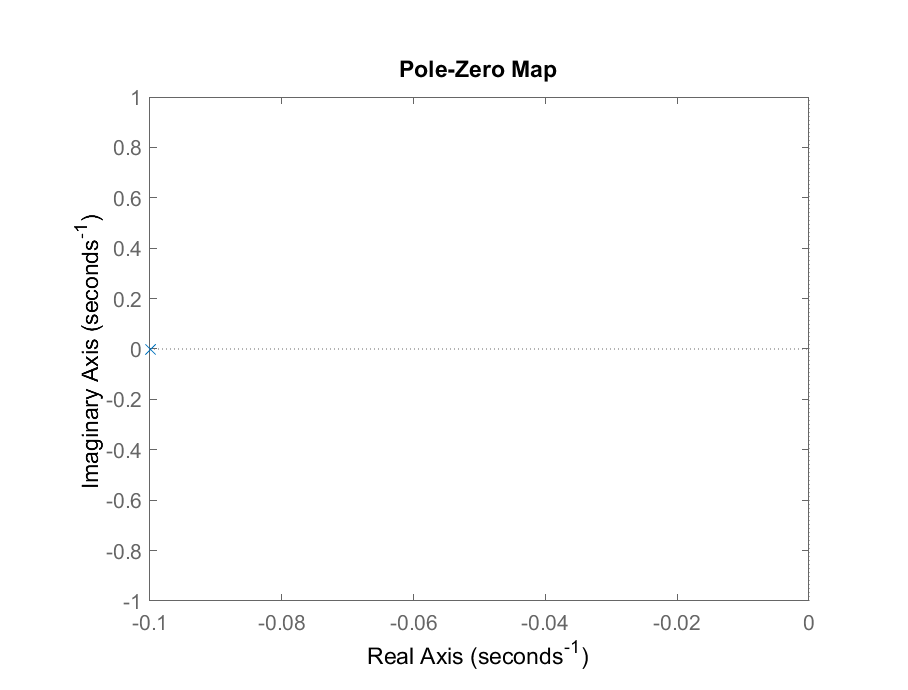
\includegraphics[width=10cm]{images_2/Rest/pzp.eps}
    \caption{Pol-Nullstellen-Plot}
\end{figure}